\section{Task 3: RF Jamming Attack}\label{ch:pentesting:rf-jamming}
This section covers a pentest of a jamming attack against the RF communication in the system. This is a \gls{DOS} attack which if successful blocks or interferes with the RF communication between two devices, making them unable to send messages to each other \cite{hacking-the-iot-talk}.

\subsubsection{Background}
Many wireless communication mediums are vulnerable to jamming attacks. Radio frequency communication is certainly one of them. In the case of RF communication, this can be likened to a \gls{DOS} attack \cite{hacking-the-iot-talk}. A jamming attack against RF communication involves directing electromagnetic energy in one or more radio frequencies against a system to disrupt or prevent signals from being transmitted between two systems \cite{adamy2004ew}. In practice, this means sending out signals on a specific frequency, carrying enough energy to overpower anyone transmission in the same frequency band. By continuously sending out signals, such that the wireless band is filled, legitimate traffic can be blocked. Since RF communication uses a shared medium, this is an attack vector that can be incredibly hard to protect against. Often a system will communicate on a single, fixed frequency which can make the system particularly vulnerable to jamming attacks \cite{jamming-feasibility}. While many sophisticated techniques to detect jamming have been developed, detection and reporting are about the extent to which a system can react to a jamming attack \cite{optimal-jamming-defense}. Little else can usually be done, except to which frequency band or fall back to an alternate mode of communication.

\subsubsection{Method}
To transmit signals the HackRF SDR was used. It was placed close to the system, within \texttt{10-20 cm}. See section \ref{ch:pentesting:lab-setup} for a detailed description of the lab setup. To generate a jamming signal the open-source program \textit{GnuRadio Companion}\footnotelink{https://www.gnuradio.org/}{2021-05-22}, version \texttt{3.9.0.0}, was used. This is a graphical tool used to control an SDR. It is based on creating flowgraphs of connected components to receive, process, modify, and transmit real-time radio signals from and to an SDR.
\begin{figure}[!ht]
    \centering
    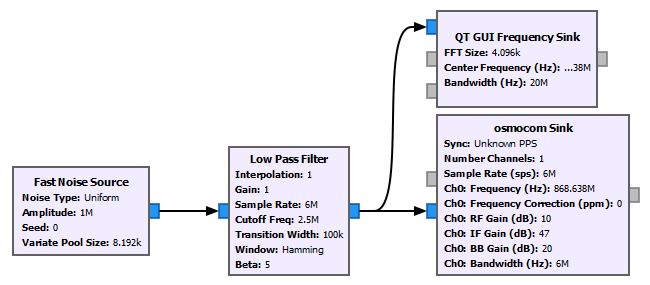
\includegraphics[width=\textwidth]{images/6-pentesting/jamming-flowgraph.png}
    \caption{A flowgraph in GnuRadio which performs a jamming attack.}
    \label{fig:gnuradio-jamming-flowgraph}
\end{figure}

To generate a noise signal, a flowgraph was created in GnuRadio Companion, see figure \ref{fig:gnuradio-jamming-flowgraph}. Initially, a \texttt{Fast Noise Generator} was used as the source signal. The noise output was then linked to a low-pass filter, to concentrate the signals to the specific frequency band of interest. Lastly, the output was sent to the HackRF via the \texttt{osmocom Sink} block. Additionally, the output from the low-pass filter was also sent to a \texttt{QT GUI Frequency Sink} to visually present the sent signal data while performing the attack. This is shown in figure \ref{fig:gnuradio-frequency-graph}.
\begin{figure}[!ht]
    \centering
    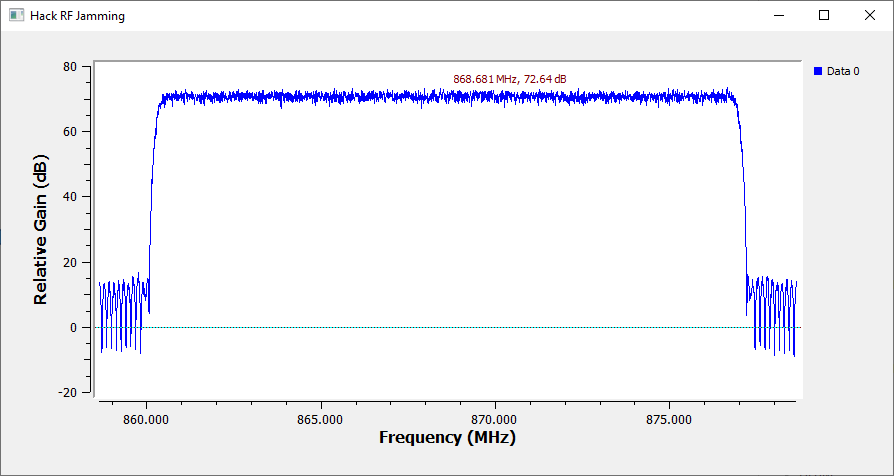
\includegraphics[width=\textwidth]{images/6-pentesting/jamming-output-graph.png}
    \caption{A frequency graph from GnuRadio during the jamming attack.}
    \label{fig:gnuradio-frequency-graph}
\end{figure}

\subsubsection{Results}
This pentest was successful. Signals between the devices were jammed, leaving the system unable to communicate. However, after approximately 60 seconds of running the attack, the main panel triggered an \textit{interference fault event}. While this fault event is triggered and the jamming attack is successfully detected by the system, crucially the event is not logged in the mobile or web application. No notification is sent to the owner of the system whatsoever.

\subsubsection{Discussion}
As expected, the system fails to communicate during the jamming attack. However, the system successfully detects this attack. Arguably, reasonable and appropriate measures have been taken by the manufacturer in this case. Given the inherent vulnerability of jamming attacks in a shared and open medium like radio frequencies, detecting and reporting is the only reasonable course of action 
\cite{optimal-jamming-defense}. This behavior in the system is documented in the official user manual submitted to the FCC \cite{hsgw-user-manual} by Climax Technology. It describes in the \textit{interference} status in section 6.1 of the manual that if a jamming period of 30 seconds or more during a one-minute window is detected then the event is triggered. This lines up with the behavior observed during the test. However, the system fails to log and report the attack to the user. This could potentially let an attacker jam the signal and do a malicious act without the user being notified. Additionally, the parameters of the jamming detection could be questioned. Letting an attacker potentially block \texttt{49\%} of the communication channel might still disturb the system significantly and potentially block important communication.

In this test the most basic jamming technique was used, e.g to send out as much noise as possible at the correct frequency band of as high energy as possible. This makes the attack quite trivial to detect. There exist much more sophisticated jamming attacks, taking less of a brute force approach, which could potentially evade detection and yet still be effective \cite{mpitziopoulos2009survey}. These, however, were considered outside the scope of this test and this report. Additionally, in this test the jamming device (the SDR) was placed very close to the system. In a real world application of this attack, the attacker would be at least a few meters away, blocked by a door. It is doubtful an SDR like the HackRF could generate enough noise to jam the system in those conditions. However, more powerful jammers, using dedicated hardware, could most likely successfully block the systems communication even in those conditions.
